\chapter{Thesis project: A standard MLOps CI/CD workflow}\label{ch:thesis-project:-a-standard-mlops-ci/cd-workflow}
\chaptermark{Thesis : MLOps WorkFlow}
\section{Introduction}\label{sec:introduction}
Following our state-of-the-art research we wanted to describe and implement a standard MLOps workflow.
I should be easily used on current project to improve their level of maturity or to initiate a new project with a solid
base to be fast in production.

We don't want to create a platform, but we want to use and integrate together reviewed
tools and workflows we encountered in the literature to propose our own.

\section{Tools}\label{sec:tools2}
In this section we will list all the tools we picked from our previous research.
As our workflow should be standard it should remain tools agnostic.

\subsection{Git Repositories and CI/CD}\label{subsec:github}
GitHub will be used to store and version control our codes repositories and configurations.
It will also be used to implement our CI/CD pipelines with GitHub actions.

\subsection{IAC, Containers and Registry}\label{subsec:dockerhub}
To benefit from containerization we will use docker to containerize our applications and models.
DockerHub will be used to store and version our Docker containers and Helm charts.

\subsection{Kubernetes}\label{subsec:kubernetes}
We will use a kubernetes cluster to benefit from its orchestration and deployment strategies and the other tools available
on kubenrets

\subsection{Airflow}\label{subsec:airflow}
We will use Airflow for our DataOps pipelines and to integrate our kubeflow pipelines.
We can use an Airflow DAG to trigger our Kubeflow pipelines and have a complete DataOps/MLOps pipeline while still allow respective teams
to benefit from other tools.

\subsection{Kubeflow}\label{subsec:kubeflow}
We will mainly use the storage solutions and pipelines offered by Kubeflow.
But by using kubeflow pipelines we could easily add features during the development.

\subsection{ArgoCD}\label{subsec:argocd}
ArgoCD will be used to implement our GitOps strategy and deploy our application, models, airflow and kubeflow.

\section{Infrastructure and Workflow}\label{sec:infrastructure}

Having established the tool requirements, we now detail the implementation of our workflow along with the minimal infrastructure necessary to sustain it.

In figure~\ref{fig:project-infra}, we describe our infrastructure that can be first deployed on a local kubernetes single node cluster
with independent DataOps and MLOps pipelines develop by potentially different teams with different roles.

\begin{figure}[!htbp]
    \centering
    \caption{Proposed MLOps kubernetes infrastructure using GitOps principles}
    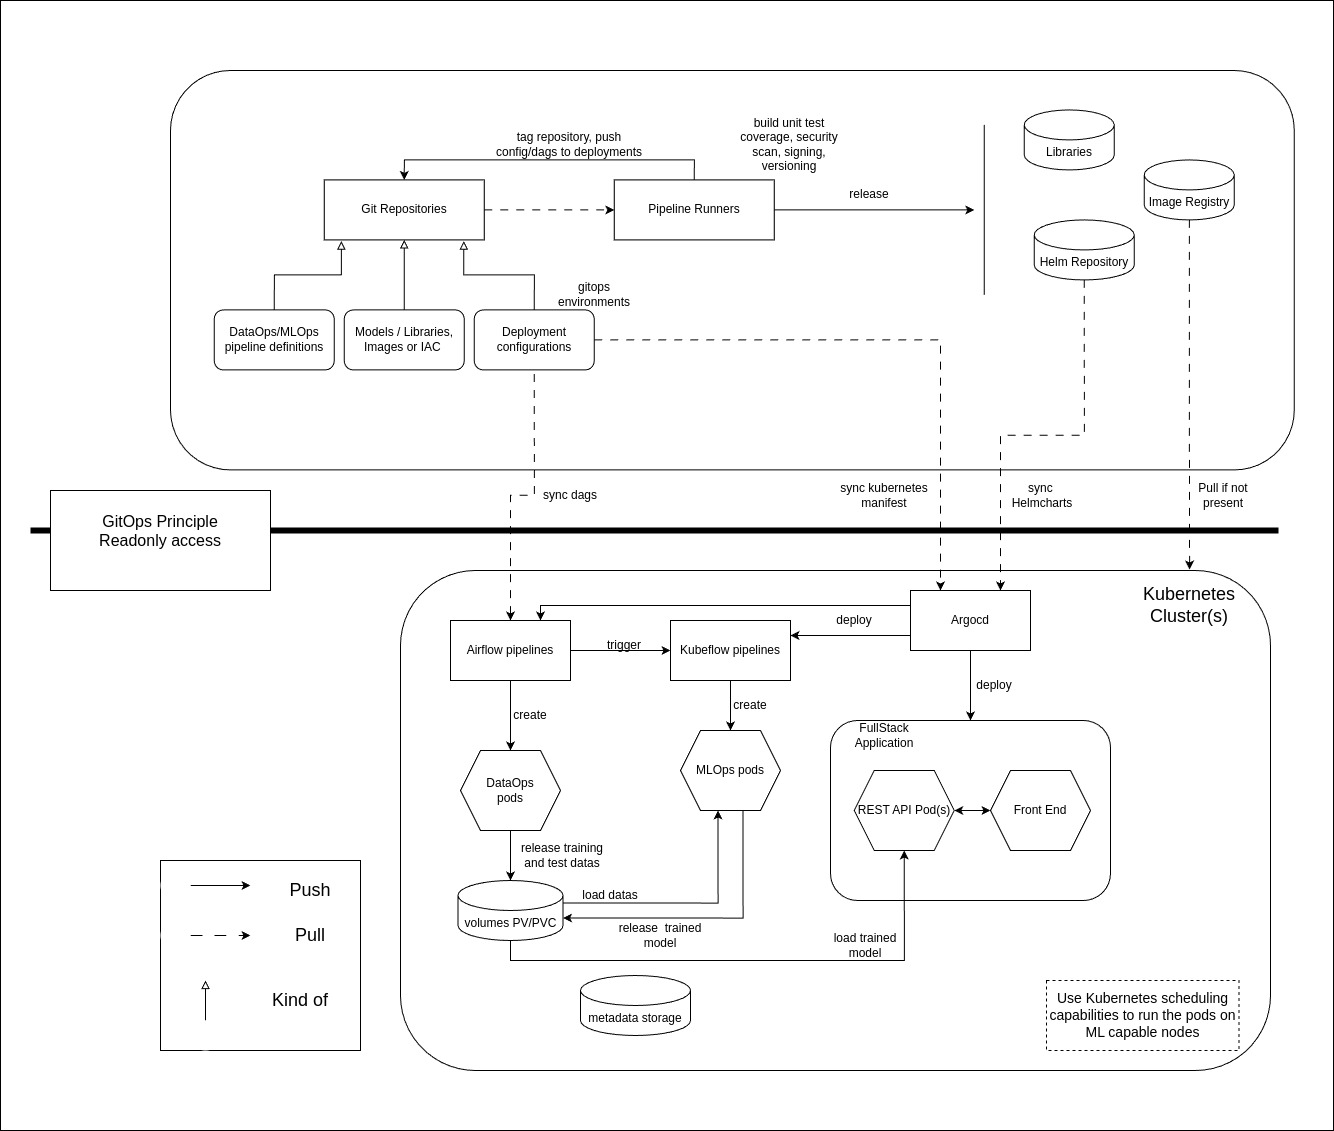
\includegraphics[scale=0.35]{images/project/mthmlops-infra}
    \label{fig:project-infra}
\end{figure}

By using Airflow pipelines as general pipelines to trigger our Kubeflow pipelines, we can easily gain in maturity towards
more automation by combining the DataOps pipelines and MLOps pipelines together when they are mature enough.

This way we enable kubeflow features for our model developers within a more general purpose environment.

By using the git-sync capabilities of Airflow we can synchronise our dags directly with airflow and
even trigger them automatically in a later stage towards automation.

Notably our infrastructure shows the GitOps pull based strategy.
Only the GitHub actions runners do pushes to other git repositories or other
storage like HelmChart repository, images repository or any library repository.
Our Kubernetes environments only pull changes from those repositories, making our infrastructure fully private and easily deployable anywhere.
We will now further describe the component of our workflow.

\subsection{General workflow}\label{subsec:general-development-workflow}
As previously outlined in our state-of-the-art review, the primary triggers for initiating our workflow are either
the emergence of a new development need or the availability of new data.
Beyond the initial phase—during which the project is discussed and defined in collaboration with business stakeholders.
The motivation for further development or model retraining typically arises from the system's monitoring and feedback loops.

Within our GitOps-based MLOps workflow, any change whether in code or configuration must be committed to the appropriate Git repository.
Each push to the repository triggers a DevOps pipeline, which culminate in updating configuration files in a dedicated configuration repository.
This repository is continuously monitored and synchronised by ArgoCD or Airflow, which applies the changes to the cluster and initiates the DataOps pipeline
or integration tests.
Upon successful completion of this stage, the MLOps pipeline is triggered.
If the newly trained model passes validation criteria, it is released to a model repository.
In accordance with GitOps principles, the deployment involves updating configuration files in a separate Git repository,
enabling ArgoCD to automatically deploy the new model version to the production environment thus closing the automation loop
as shown in figure~\ref{fig:general-workflow}.

\begin{figure}[!htbp]
    \centering
    \caption{General Workflow}
    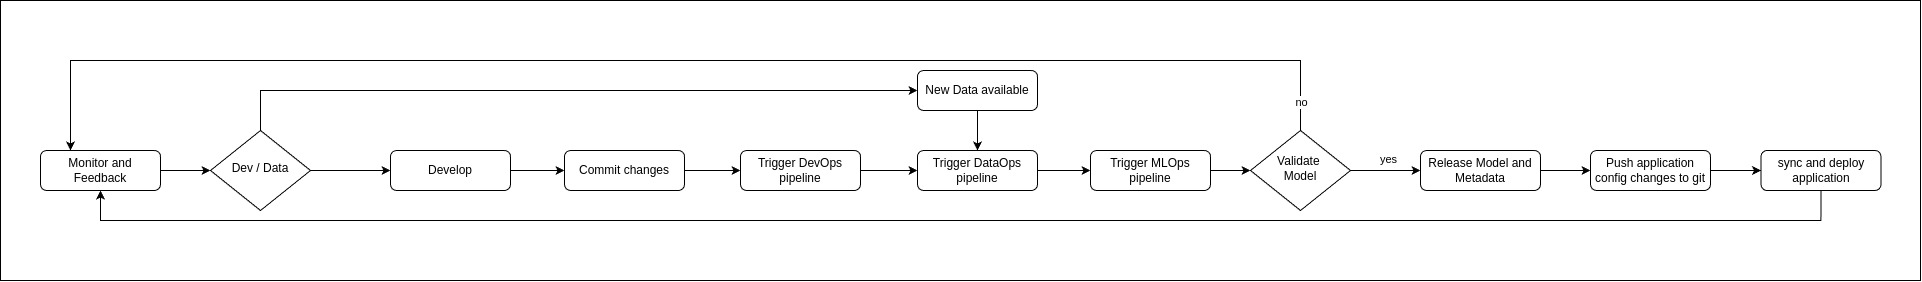
\includegraphics[width=\linewidth]{images/project/general_workflow}
    \label{fig:general-workflow}
\end{figure}

\subsection{Git Repositories}\label{subsec:git-repositories}
As we said, we use Git Repositories for version control and triggering our DevOps pipelines.

Within our infrastructure, we consider 4 types of Git Repositories:

\begin{itemize}
    \item Code Repositories that holds code for models, libraries, docker images and infrastructure as code using Helm.
    \item MLOps and DataOps Pipelines Repositories.
    In our infrastructure those repositories holds the definition of our Airflow DAGs.
    In the first iteration those repositories can also hold images for.
    \item Deployment/Configuration repositories.
    Those repositories are used to hold configuration for the deployed applications and Airflow dags.
    We use ArgoCD GitOps implementation to synchronise changes to those repositories.
    Airflow git/sync feature allows us to synchronise our dags with
    Change in those repositories can be automated by the pipeline runners.
    Depending on your team and organization those repositories can be separated into multiple repositories (per team, per domain, per environment (dev,test,staging,prod))
    For the Dev environment we allow developers to push from their code repositories within those repositories.
    For the production environment we use a pipeline to pull the configuration from the staging environment.
    We called this promote our configuration to a new environment.
    In case of full automation the pulling/promotion can be trigger automatically by ArgoCD sending webhooks on any test results desired.
    \item CI/CD pipelines templates
    In those we define workflows that can be used in any repository to be used by the developers.
    It includes building image workflows, versioning with tags on repositories, pushing new configurations into deployments repositories.
    By defining them in a separate repository it allows us to version them and make it easy for developers to choose a workflow.
    Each workflow is closely tight to the structure of the repository, so we defined one per type of repositories.
\end{itemize}

Following GitOps principle those are the source of truth for all our code and configurations, for the infrastructure, the pipelines, the model and the software development.
We adopt a consistent structure (figure~\ref{fig:sidebyside}) for both our DataOps and MLOps pipeline repositories, incorporating a config.yml file that mirrors the organizational pattern of Helm chart project (values.yaml).
In both cases, an images directory is used to define containerized steps for the pipelines and for deployment configurations within the Helm charts.
This consistency permit to reuse our Devops pipelines templates.

\begin{figure}[h!]
    \centering
    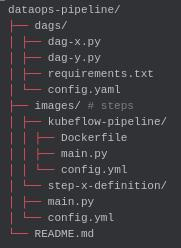
\includegraphics[scale=0.35]{images/project/git-repo-dataops}
    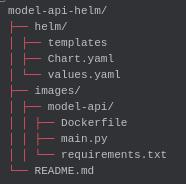
\includegraphics[scale=0.35]{images/project/git-repo-helm}
    \caption{Consistent structure within repositories}
    \label{fig:sidebyside}
\end{figure}


\subsubsection{General Rules for Managing Git Repositories}
We follow the GitHub flow with adaptations to fit our workflow.
However, it can be adjusted as needed.

\begin{itemize}
    \item A Pull Request is required for merging into the \texttt{main} branch, including a pipeline run and team review.
    \item Follow GitHub flow, using \texttt{feature/} and \texttt{hotfix/} branches for development.
    \item Approvals are required for deploying to environment-specific repositories.
    \item The \texttt{main} branch is deployed to the production environment or released into production Docker/Helm repositories.
    \item Other branches are deployed sequentially to all environments, passing tests and approval gates before merging to main.
\end{itemize}

\subsection{GitOps}\label{subsec:gitops2}
With a Helm-based installation pipeline, the runner requires write access to push applications directly to Kubernetes.
By adopting ArgoCD and a GitOps approach, we eliminate this requirement by pulling changes directly from GitHub.
This enables all operations to be managed within GitHub.
However, it necessitates properly configured permissions in GitHub to prevent potential security breaches.

Airflow also integrate a Git/Sync feature that allows us to load and trigger the DAGs within Airflow.

\subsection{DataOps pipelines}\label{subsec:dataops-pipelines2}
DataOps pipelines are defined as Airflow DAGs that will, with the KubernetesExecutor functionality of Airflow,
create pods for every step defined in the pipeline.
They can be connected to an observability stack like OpenSearch or Elasticsearch to analyse and store the data.
Those can be used as Monitoring tools for all our infrastructure too.

\begin{figure}[!htbp]
    \centering
    \caption{Example of a DataOps pipeline define within Airflow}
    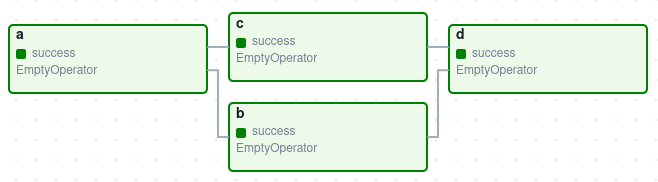
\includegraphics[scale=0.5]{images/project/data-ops-airflow-dag}
    \label{fig:project-data-ops-airflow-dag}
\end{figure}

\subsection{MLOps pipelines}\label{subsec:mlops-pipelines2}
Kubeflow allows us to deploy all the required steps within our MLOps pipeline by creating pods in the required namespace within our Kubernetes cluster.
A lot like Airflow would.
We use Kubeflow to allow our ML engineer to use other features like model and metadata storage.
Other features from the Kubeflow ecosystem could be added at any time if necessary.

\begin{figure}[!htbp]
    \centering
    \caption{Example of a MLOps pipeline define within Airflow}
    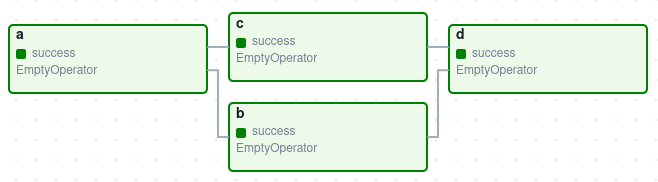
\includegraphics[scale=0.5]{images/project/data-ops-airflow-dag}
    \label{fig:project-ml-ops-airflow-dag}
\end{figure}

\subsection{Storage}\label{subsec:storage}
Here we detail the storage found in our infrastructure (\ref{fig:archi}) and their purpose in our workflow.

\begin{itemize}
    \item Model repository manage by Kubeflow to store our trained, pretrained and untrained models.
    It's an S3 storage that can be mounted as a volume in kubernetes and attached to a running container.
    \item Image repository where we store our container images to be pull by our cluster during deployment.
    \item HelmChart repository to hold and version our infrastructure-as-code templates as packages.
    \item Metadata Database manage by Kubeflow to store model metadata and experiment tracking info.
    \item Git repositories to store code and configuration as already stated.
\end{itemize}

\subsection{Model development}\label{subsec:model-development}
As previously mentioned, we use Helm and Docker to package our model code.
In this section, we'll go into detail about how the model is defined.
The model's Docker image supports three operational modes, each configurable via parameters:
\begin{itemize}
    \item Training mode that loads and trains the untrained model on training data.
    \item A validation mode to load, test and validate the model.
    \item A listen mode define as a REST API server to interface with external frontends or services.
\end{itemize}

To integrate smoothly with our DataOps and MLOps pipelines, we define parameters that specify storage locations.
This ensures that any container image meeting these requirements can be seamlessly used within the pipeline.
Since we use the container layered model, it allows us to take any base image and add a layer that satisfies our pipeline's interface requirements.
While it's convenient to define all stages (training, validation, and listening) within a single image, it may be preferable to split them into two or three separate images.
One downside of the single-image approach is that the model's code is packaged into the same container that's deployed to production.

To deploy our production REST API server to Kubernetes, we created a standard Helm project with template manifests for a Service,
ServiceAccount, Ingress, and Deployment.
In the Helm (values.yaml) configuration file, we specify which trained model version should be loaded, allowing for seamless model hot-swapping when needed.
For more advanced deployment strategies, we can replace the standard Deployment manifest with a Rollout manifest (Custom Resource Definition (CRD) managed by Argo Rollouts).

To use the model within our MLops Kubeflow pipeline, we use our training and validation mode and our data location parameters with Kubeflow Domain specific language container components.
We use the same approach for our DataOps pipelines steps to ensure consistency as we'll demonstrate later in this paper.

% image de argocd api deployment.




\section{Workflow}\label{sec:workflow}
As we explained while describing the infrastructure, part of our global workflow can be implemented within pipelines runners definition.
We used GitHub action and the GitHub flow to harmonise the workflow within our different type of git repositories.
GitHub allows us to define template in a single repository that can be then versioned and used in other repositories while hiding the complexity of the defined pipelines.



\section{Conclusion}\label{sec:conclusion}
Airflow pipelines and kubeflow pipelines to easily integrate DataOps and MLOps pipelines together to reach more automation as the project gains maturity.
